\chapter{Validation}
\label{chaper-3}

Validation du simulateur avec exo 4 TP 1, sous forme de tableau comparatif à double entrée.....\\
Détail calcul à la main...\\
Tracé des rayons obtenus àpd simulateur...\\





Lors de la simulation de la situation de l'exercice 1 du TP4, nous ne pouvons pas utiliser la puissance sur une zone locale $<P_{RX}>$ (équation \ref{eq:puissance-locale}), mais bien $P_{RX}$ en un point de l'espace.

\section{Calculs deux réflexions, cas A}
...


\section{Comparaison calculs et simulation}
...


\begin{table}
    \centering
    \begin{tabular}{|l|l|r|r|r|}
         \hline
                                  & Grandeur & Calculs & Simulation & Erreur \\
        \hline
\multirow{2}{*}{Direct}           & $\left|\underline{E}\right|$ [V/m] & $4,031\cdot10^{-3}$ &      & \%     \\
                                  & $P_{RX}$ [W] & $3,33\cdot10^{-10}$  &      & \%     \\
        \hline
\multirow{2}{*}{1 réflexion (A)}  & $\left|\underline{E}\right|$ [V/m] & $7,0819\cdot10^{-4}$ &      & \%     \\
                                  & $P_{RX}$ [W] & $1,04\cdot10^{−11}$ &      & \%     \\
        \hline
\multirow{2}{*}{1 réflexion (B)}  & $\left|\underline{E}\right|$ [V/m] & $6,7821\cdot10^{-4}$ &      & \%     \\
                                  & $P_{RX}$ [W] & $9,53\cdot10^{-12}$ &      & \%     \\
        \hline
\multirow{2}{*}{2 réflexions (A)} & $\left|\underline{E}\right|$ [V/m] & $4,4572\cdot10^{-4}$ &      & \%     \\
                                  & $P_{RX}$ [W] & $4,11\cdot10^{-12}$ &      & \%     \\
        \hline
%\multirow{2}{*}{2 réflexions (B)} & $\left|\underline{E}\right|$ [V/m] &   N/A   &      & N/A    \\
%                                  & $P_{RX}$ [W] &   N/A   &      & N/A    \\
%         \hline
    \end{tabular}
    \caption{Comparaison valeurs calculs et simulation}
    \label{tab:comparaison-calculs-simulation}
\end{table}

\section{Affichage simulation}
...

\begin{figure}[H]
    \centering
    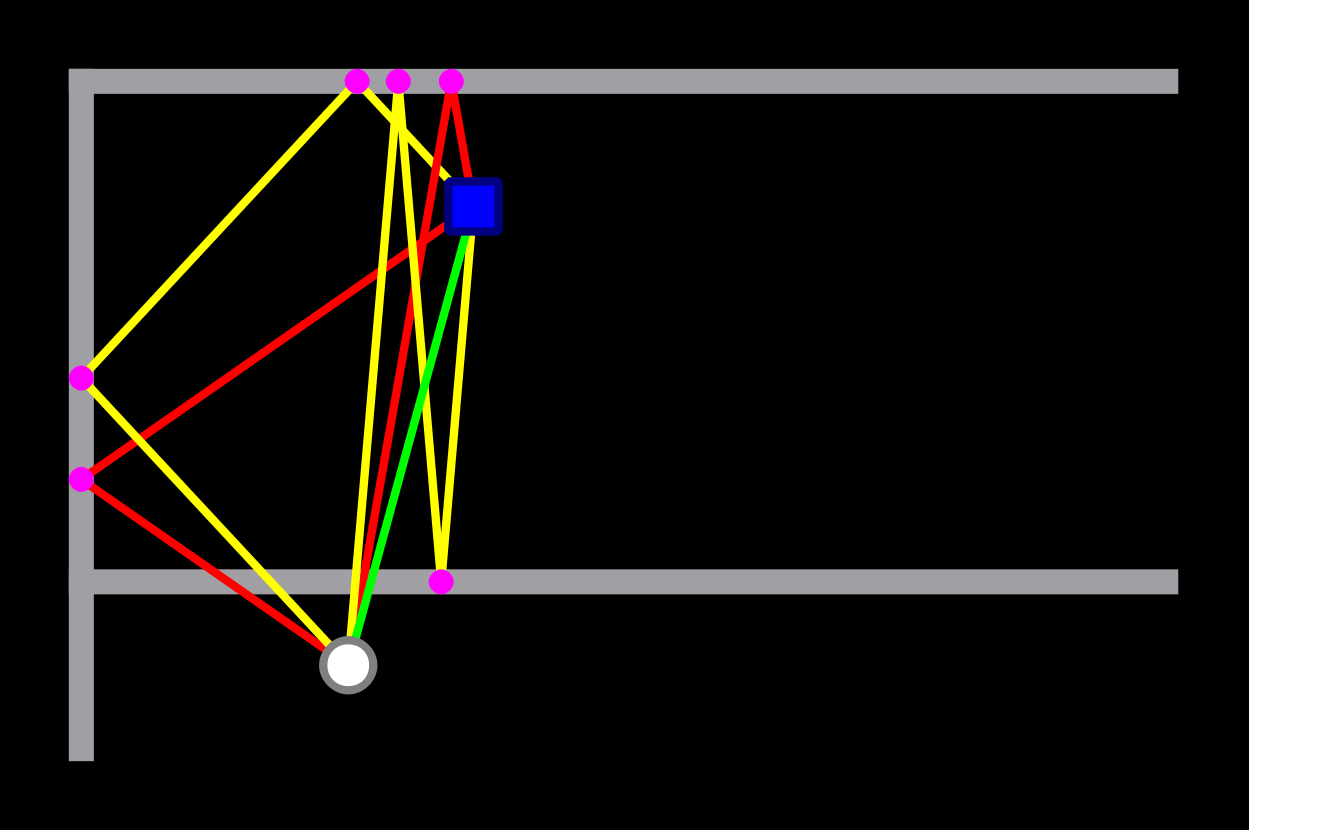
\includegraphics[width=\textwidth]{latex/images/tp4.png}
    \caption{Simulation Ray-Tracing de l'exercice 1, TP4}
    \label{fig:simu-tp4}
\end{figure}
